\documentclass{article}
\usepackage{graphicx}
\usepackage{algorithmic}
\begin{document}
\section{User Interface}
User interface is useful for taking input from  user and giving results to the user. First this module asks user to load an 
input file and passes it to parser module. After initialization of the PMs and VMs by the PM modifier module it displays a 
screen with buttons specifying the PMs and labels specifying their respective VMs.\\
It also has buttons to specify functionalities of the the system such as addVM,deleteVM,reset and consolidate. 
\begin{figure}[h]
\centering
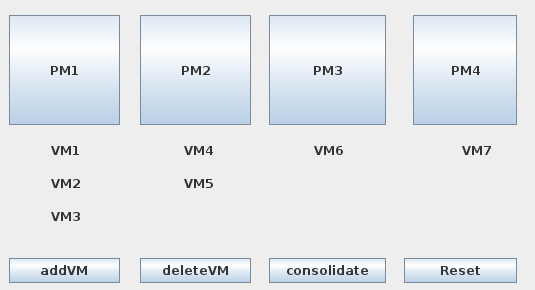
\includegraphics[height=6cm]{3.png}
\caption{User interface}
\end{figure}
\subsection{Internal Functions}
\emph{\bf callParser()}\\\\
Initially user interface has a load button.On clicking, it opens a file chooser which helps  the user to choose an input file.
\\ 
The selected input file is passed to the parser module. \\
\begin{tabbing}
\hspace*{4cm}\= \kill
\emph{Input parameters} \>: Click event \\
\emph{Output parameters} \>: File \\
\emph{Returns} \>: UI is updated on success.\\ \>If the file chosen is not in the  specified format an\\ \> error message is returned.\\
\end{tabbing}
\textbf{Pseudo code :}
\begin{algorithmic}[1]
 \STATE on clicking load
 \STATE open file chooser
  \IF {file choosen}
  \STATE call parser(file) in parser module
  \STATE call updateUI()
  \ELSE 
  \STATE no change
  \ENDIF
 \end{algorithmic}
\begin{figure}[ht!]
\centering
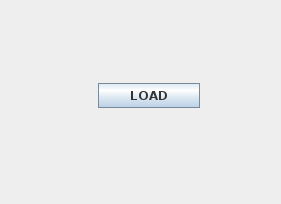
\includegraphics[height=5cm]{1.png}
\caption{Initial GUI}
\end{figure}
\begin{figure}[h]
\centering
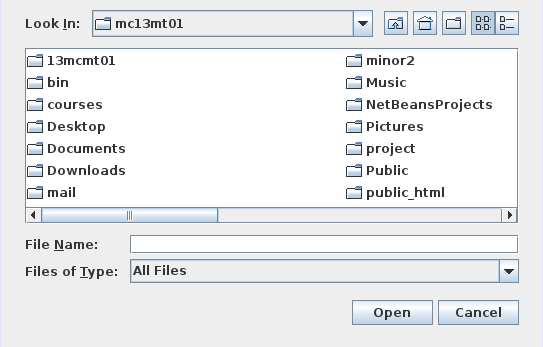
\includegraphics[height=6cm]{2.png}
\caption{File chooser}
\end{figure}
\begin{figure}[h]
 \centering
 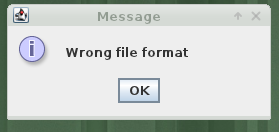
\includegraphics[height=3cm]{7.png}
 \caption{Error message}
\end{figure}
\pagebreak
\mbox{}\\\\
\emph{\bf callAddVM()}\\\\
 On click addvm button ,a window asking the user to enter VM\textunderscore ID and  capacity opens.
  Once the user specifies VM\textunderscore ID and its capacity it calls the addVM() in PM modifier module.And then calls updateUI() which is an internal function.
  \\
  \begin{figure}[ht!]
 \centering
 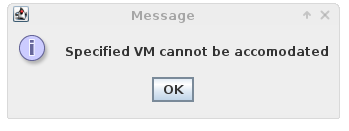
\includegraphics[scale=0.5, angle=0]{8.png}
 \caption{Error message}
\end{figure}
  \begin{tabbing}
  \hspace*{4cm}\= \kill
  \emph{Input parameters}\>: Click event\\
\emph{Output parameters}\>: VM\textunderscore ID ,Capacity\\
\emph{Returns}\>: UI is updated on success. \\ \> Error message is returned if the specified VM cannot be \\ \> accommodated by any of the PMs.\\
\emph{Error condition} \>: Entering negative numbers,alphanumerics,special \\ \> characters, numbers greater than  physical machine \\ \>capacity can be avoided by data validation.
 \\
 \end{tabbing}
  \textbf{Pseudo code :}
 \begin{algorithmic}[1]
\STATE on clicking addVM
\STATE open dialog asking for VM\textunderscore ID and capacity
\STATE input validation
\IF {valid}
\STATE call addVM(VM\textunderscore ID,capacity) in PM modifier
\STATE call updateUI()
\ELSE 
\STATE show error message
\ENDIF
 \end{algorithmic}
\mbox{}\\\\
 \emph{\bf callDeleteVM()}\\\\
 On clicking the deleteVM button in user interface, it opens a window  which prompts the user to choose a VM for deletion.
 This calls the deleteVM() in PM modifier module .Later calls an internal funtion updateUI().
 \\  \begin{tabbing}
   \hspace*{4cm}\= \kill
 
 \emph{Input parameters}\>: Click event\\
 \emph{Output parameter}\>: VM\textunderscore ID\\
\emph{Returns}\>: UI is updated on success.\\
\emph{Error conditions}\>: Choosing an incorrect VM\textunderscore ID. But this case is avoided \\ \> by listing all the VMs present in the system.
\end{tabbing}
\begin{algorithmic}[1]
 \STATE on clicking deleteVM
 \STATE open dialog displaying list of VMs ,asking user to choose VM for deletion
 \IF {choosen}
 \STATE call deleteVM(VM\textunderscore ID)
 \STATE call updateUI()
 \ELSE
 \STATE do nothing
 \ENDIF
 \end{algorithmic}
\begin{figure}[ht!]
\centering
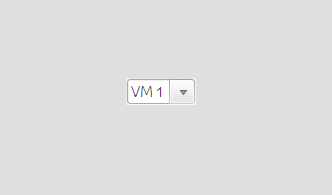
\includegraphics[scale=0.8, angle=0]{4.png}
\caption{VM Deletion}
\end{figure}
\mbox{}\\\\
\emph{\bf callConsolidate()}\\\\
On clicking consolidate button in UI it opens a window for confirmation from the user \\
If the user chooses not to consolidate the state of the system does not change.\\
If the user chooses to consolidate ,  then conolidate() funtion in PM modifier is called.
\\ The user interface is updated using the updateUI() function.
\\
  \begin{tabbing}
  \hspace*{4cm}\= \kill
\emph{Input parameters}\>: Click event
\\
\emph{Output parameters}\>: None \\
\emph{Returns}\>: UI is updated and the color of the physical machines\\ \> that are switched off changes.\\
\emph{Error condition} \>: None\\
\end{tabbing}
\textbf{Pseudo code :}
\begin{algorithmic}[1]
\STATE on clicking consolidate
\STATE open dialog for confirmation
\IF {confirmed}
\STATE call consolidate()
\STATE call updateUI()
\ELSE 
\STATE do nothing
\ENDIF
\end{algorithmic}
\begin{figure}[ht!]
\centering
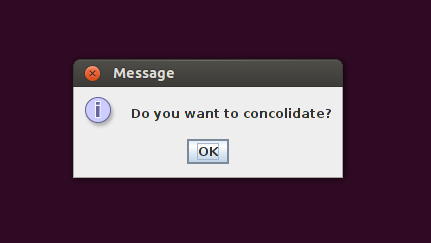
\includegraphics[scale=0.6, angle=0]{5.png}
\caption{Consolidation}
\end{figure} 
\mbox{}\\\\
\textbf{ callReset()}\\\\
On clicking reset button in user interface, a window opens for confirmation from the user.\\
If the user chooses to reset then all the VMs in the present system are deleted and  a new input is loaded again.\\
If the user does not wish to reset, then there is no change in  state of the sytsem. \\
  \begin{tabbing}
  \hspace*{4cm}\= \kill
\emph{Input parameters}\>: Click event \\
\emph{Output parameters}\>: None \\
\emph{Return values}\>: Updated UI\\
\emph{Error conditions}\>: None\\
\end{tabbing}
\textbf{Pseudo code :}
\begin{algorithmic}[1]
\STATE on clicking reset
\STATE open dialog for confirmation
\IF {confirmed}
\STATE call reset() in PM modifier
\STATE call updateUI()
\ELSE 
\STATE do nothing
\ENDIF
\end{algorithmic}
\begin{figure}[ht!]
\centering
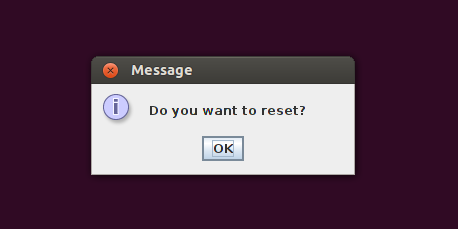
\includegraphics[scale=0.6, angle=0]{6.png}
\caption{Reset}
\end{figure} 
\mbox{}\\\\
\emph{\bf updateUI()}\\\\
This function is called after every change performed on the system to reflect changes to the user.It calls the status() function in PM modifier module.
\\\begin{tabbing}
  \hspace*{4cm}\= \kill

\emph{Input parameters}\>: None
\\
\emph{Output parameters}\>: None\\
\emph{Returns}\>: Updated UI\\
\emph{Error conditions}\>: None\\
\end{tabbing}
\textbf{Pseudo code :}
\begin{algorithmic}[1]
 \STATE call status()
 \STATE accordingly modify PMs and VMs
\end{algorithmic}
\mbox{}\\\\
\emph{\bf OnPM()}\\\\
This function is used to switch on a PM manually by the user.When user clicks a PM  which is in off state,changes its state to ON by calling the switchOnPM() function in PM modifier.Then calls updateUI().
If user chooses a PM that is already in on state ,a message is prompted to user if he/she wishes to turn off respective PM
\\\begin{tabbing}
  \hspace*{4cm}\= \kill
\emph{Input parameters}\>: Click event\\
\emph{Output parameters}\>: PM\textunderscore ID\\
\emph{Returns}\>: UI is updated on success.The color of the PM that is \\ \> turned on changes.On failure returns an error message.\\ 
\end{tabbing}
\textbf{Pseudo code :}
\begin{algorithmic}[1]
 \STATE on clicking PM 
 \IF {PM in OFF state}
 \STATE OPEN DIALOG FOR CONFIRMATION
 \IF {confirmed}
 \STATE call switchOnPM() in PM modifier
 \ELSE 
 \STATE no change
 \ENDIF
 \ENDIF
\end{algorithmic}
\mbox{}\\\\
\emph{\bf OffPM()}
\\\\
This function is used to switch off a PM manually by the user.When user clicks a PM which is turned on,changes its state to OFF by calling switchOffPM() function in PM modifier.
\\\begin{tabbing}
  \hspace*{4cm}\= \kill
  \emph{Input parameters}\>: Click event\\
  \emph{Output parameters}\>: PM\textunderscore ID\\
  \emph{Returns}\>: UI is updated on success.The color of the PM that is \\ \> turned off changes.On failure returns an error message.\\
  \emph{Error conditions}\>: If the VMs in selected PM cannot be accommodated in another PMs.
  \end{tabbing}
  \textbf{Pseudo code :}
  \begin{algorithmic}[1]
   \STATE on clicking PM 
   \IF {PM is in ON state}
   \STATE open dialog for confirmation
   \IF {confirmed}
   \STATE call switchOffPM()
   \IF {no error}
   \STATE call updateUI()
   \ELSE 
   \STATE show error message
   \ENDIF
   \ELSE
   \STATE no change
   \ENDIF
   \ENDIF
  \end{algorithmic}


\end{document}
